\chapter{Coordinación con Crazyflies}

Conseguido el funcionamiento de GVF para un Crazyflie, 
se extenderá este funcionamiento de forma que dos o más Crazyflies sean coordinables,
es decir, que los recorridos que estos realicen tengan algún tipo de coordinación y dependencia mutua. Dicho de otro modo, formaciones de drones.

%%%%%%%%%%%%%%%%%%%%%%%%%%%%%%%%%%%%%%%%%%%%%%%%%%%%%%%%%%%%%%%%%%%%%%%%%%%%%%%%%%%%%%%%%%%%%%%%%%%%%%%%%%%%%%%%%
%%%%%%%%%%%%%%%%%%%%%%%%%%%%%%%%%%%%%%%%%%%%%%%%%%%%%%%%%%%%%%%%%%%%%%%%%%%%%%%%%%%%%%%%%%%%%%%%%%%%%%%%%%%%%%%%%
%%%%%%%%%%%%%%%%%%%%%%%%%%%%%%%%%%%%%%%%%%%%%%%%%%%%%%%%%%%%%%%%%%%%%%%%%%%%%%%%%%%%%%%%%%%%%%%%%%%%%%%%%%%%%%%%%

\section{Algoritmos de coordinación}

El algoritmo de coordinación elegido es una extensión de GVF para 
poder realizar formaciones circulares \cite{circular-formations}.
Además, se propone una variante de este algoritmo para poder realizar 
GVF coordinado en segmentos paralelos.

\subsection{Formación circular}

Se empezará dando un resumen de la formalización matemática dada por \cite{circular-formations}.
Para ello, se recomienda entender las nociones matemáticas de GVF previamente descritas en el capítulo 3.

Sea un conjunto de vehículos $n \in \mathbb{N}$ tal que $n \geq 2$ cuyas posiciones estan definidas por
$p_i \in \mathbb{R}^2$ para $i \in \{1 \ldots n\}$ se define el grafo no dirigido
$\mathcal{G} = \{\mathcal{V}, \mathcal{E}\}$ donde $\mathcal{V} = \{1 \ldots n \}$ es el conjunto de vértices
y $\mathcal{E} \subseteq \mathcal{V} \times \mathcal{V}$ es el conjunto de aristas.
De este grafo, nos interesa la  matriz de incidencia 
$B \in \mathbb{R}^{|\mathcal{V}| \times |\mathcal{E}|}$ que es definida de la siguiente forma:

\begin{equation}
    b_{ik} \triangleq 
    \begin{cases} 
        +1 \ para \ i = \mathcal{E}^{tail}_{k} \\
        -1 \ para \ i = \mathcal{E}^{head}_{k}  \\
        0 \ en \ otro \ caso
    \end{cases}
\end{equation}

Donde $\mathcal{E}^{tail}_{k}$ y $\mathcal{E}^{head}_{k}$ son los nodos finales e iniciales 
de una arista $\mathcal{E}_{k} = (\mathcal{E}^{tail}_{k}, \mathcal{E}^{head}_{k})$.

Con esta matriz de incidencia, podemos realizar una topología de enlaces entre vehículos de forma que
visualmente se pueda ver en la matriz que UAV toma como referencia un UAV dado.
Esto cobrará más sentido conforme se avance en esta subsección. 

Recordemos que al estar en un entorno GVF para círculos, nuestras curvas de nivel se rigen por la ecuación
$\varphi(p) = p_{x}^2 + p_{y}^2 - r^2$ donde $r \in \mathbb{R}^+$ es el radio.

Por otro lado, la coordinación se realizará en base a un ángulo, es decir, cuanto ángulo hay de desfase entre un vehículo y otro. 
Por ello, el ángulo de un vehículo $i$ en un punto $p$ respecto a $\mathcal{O}_\mathcal{N}$
del plano $\mathbb{R}^2$ viene dado por \cite{atan2}:

\begin{equation} \label{eq:theta-circular-formation}
    \theta_i(p) = atan2(p_y, p_x) \in (-\pi, \pi]
\end{equation}

Evidentemente, los ángulos que más interesan son los que hay entre un vehículo y otro, 
no el ángulo respecto a el origen de coordenadas $\mathcal{O}_\mathcal{N}$, 
solo se necesitan para calcularlos. 
Para ello, los autores de \cite{circular-formations} proponen calcular un vector de ángulos entre vehículos de la siguiente forma:

\begin{equation}
    z = B^T\theta
\end{equation}

Donde $\theta$ es el vector de ángulos calculados usando la \autoref{eq:theta-circular-formation}
y $z = \{z_1 \ldots z_k\}, \ k = |\mathcal{E}|$ es el vector de ángulos entre vehículos.
Supóngase ahora un conjunto de ángulos deseados $z^{*}_{k}$, se define $e_\theta$ como el conjunto de error
entre el ángulo actual y el deseado, regido por la ecuación:

\begin{equation}
    e_{\theta_k}(t) = z_k(t) - z_k^*
\end{equation}

Se desea que $e_\theta(t) \to 0$ para $t \to \infty$

Con toda esta base, los autores de \cite{circular-formations} terminan proponiendo la siguiente 
ecuación para control y coordinación.

\begin{equation} \label{eq:control-action-circular-formation}
    ^iu_r = k_r B_i e 
\end{equation}

Donde:

\begin{itemize}
    \item $B_i$ es la i-ésima fila de la matriz de incidencia
    \item $e$ es el vector de errores entre ángulos de vehículos
    \item $k_r \in \mathbb{R}^+$ es una ganancia de control para ajustar el resultado final  
    \item $^iu_r$ es la acción de control resultante para el radio $r$ del vehículo $i$
\end{itemize}

Finalmente, se aplica sobre el vehículo la acción de control de forma que el 
radio nuevo sea tal que permita, bajo \textbf{velocidad constante}, que los 
vehículos vayan convergiendo al ángulo deseado. 
Por tanto, aplicamos lo siguiente para cada vehículo $i$:

\begin{equation} \label{eq:applied-control-action-circular-formation}
    r_i = r_i + {^iu_r}
\end{equation}

Resumidamente, el algoritmo consiste en:

\begin{itemize}
    \item Definir un grafo $\mathcal{G}$ y usar su matriz de incidencia $B$ para definir que drones 
    se coordinarán entre sí
    \item Calcular el vector de ángulos entre vehículos $z$ en base al vector de ángulos $\theta$ respecto a 
    $\mathcal{O}_\mathcal{N}$ del plano $\mathbb{R}^2$
    \item Calcular el vector de error entre ángulos de vehículos $e$ en base a $z$ y 
    un vector de ángulos deseados $z^*$
    \item Calcular las acciones de control $u_r$ en base a $e$, $B$ y una ganancia de control $k_r$
    \item Aplicar la acción de control $u_r$ al radio actual $r$
\end{itemize}

Por simplicidad, se han obviado ciertas demostraciones, pasos y definiciones. 
Si se desea profundizar, se recomienda leer \cite{gvf-hector} y \cite{circular-formations}.

\subsection{Formación en segmentos paralelos}

La formación en segmentos paralelos consistirá en dos o más UAVs 
cada uno siguiendo su propio segmento que serán paralelos entre sí.
Es preferible usar segmentos de misma longitud.
Por simplicidad en la implementación, 
se realizará una aplicación de los segmentos de -1 a 1, 
siendo -1 un extremo y 1 el opuesto como en la figura:

\begin{figure}[!h]
    \centering
    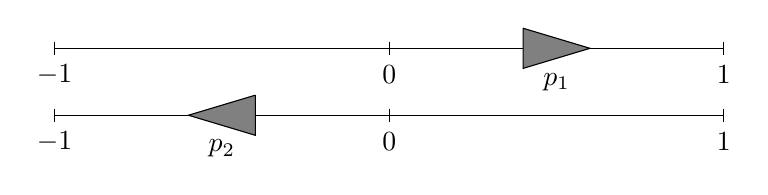
\begin{tikzpicture}[scale=0.85]
        % Dibujar el segmento de -1 a 1
        \draw[-] (-5,0) -- (5,0);
        
        % Poner las etiquetas en los extremos y en el centro
        \node at (-5, -0.4) {$-1$};
        \node at (0, -0.4) {$0$};
        \node at (5, -0.4) {$1$};
        
        % Poner las marcas en los puntos -1, 0 y 1
        \draw[-] (-5,0.1) -- (-5,-0.1);
        \draw[-] (0,0.1) -- (0,-0.1);
        \draw[-] (5,0.1) -- (5,-0.1);

        % Dron 1
        \draw[fill=gray,cm={cos(0),-sin(0),sin(0),cos(0),(0,0)}](2,0.3)--(2,-0.3)--(3,0)--(2,0.3);
        \node at (2.5, -0.5) {$p_1$};
        
        % Segundo Segmento
        % Dibujar el segmento de -1 a 1
        \draw[-] (-5,-1) -- (5,-1);
        
        % Poner las etiquetas en los extremos y en el centro
        \node at (-5, -1.4) {$-1$};
        \node at (0, -1.4) {$0$};
        \node at (5, -1.4) {$1$};
        
        % Poner las marcas en los puntos -1, 0 y 1
        \draw[-] (-5,-0.9) -- (-5,-1.1);
        \draw[-] (0,-0.9) -- (0,-1.1);
        \draw[-] (5,-0.9) -- (5,-1.1);

        % Dron 2
        \draw[fill=gray,cm={cos(0),-sin(0),sin(0),cos(0),(0,0)}](-2,-0.7)--(-2,-1.3)--(-3,-1)--(-2,-0.7);
        \node at (-2.5, -1.5) {$p_2$};
    \end{tikzpicture}
    \caption{Ejemplo de segmentos paralelos y normalizados para dos drones}
    \label{fig:parallel-segments-formation}
\end{figure}

Para realizar formación coordinada en segmentos paralelos, este trabajo
se basará en el modelo Kuramoto \cite{kuramoto-model}.
El modelo de Kuramoto se utiliza para describir la sincronización de sistemas oscilatorios 
bajo la siguiente ecuación:

\begin{equation}\label{eq:kuramoto}
    \frac{d\theta_i}{dt} = \omega_i + \frac{K}{N} \sum_{j=1}^{N} sin(\theta_j - \theta_i), 
    \ \ \ \ \ i = 1 \ldots N
\end{equation}

En base a esta ecuación y la \autoref{fig:parallel-segments-formation}, 
se propone la siguiente versión adaptada para el control en segmentos paralelos:

\begin{equation}\label{eq:segment-formation}
    v_i = v_n + K \sum_{j=1}^{N} (p_j - p_i - p^{*}_{ij}), 
    \ \ \ \ \ i = 1 \ldots N
\end{equation}

Donde:

\begin{itemize}
    \item $v_i \in \mathbb{R}$ es la velocidad resultante para el dron $i$
    \item $v_n \in \mathbb{R}$ es la velocidad nominal (o velocidad base) de los drones
    \item $K \in \mathbb{R}$ es la ganancia
    \item $N \in \mathbb{N}$ es el número total de drones
    \item $p_i$ es la posición del dron sobre el segmento normalizado, 
    por tanto $p_i \in [-1, 1], \ \forall i$
    \item $p^{*}_{ij}$ es el desajuste de la posición deseado entre el dron $i$ 
    y el dron $j$ que valdrá entre $[-2, 2]$. Por ejemplo, para 0, 
    se tiene que los drones han de estar uno al lado del otro y en paralelo.
\end{itemize}

Intuitivamente, podemos comprender el siguiente algoritmo para el caso 
$N = 2, \ K = 1, \ p^{*}_{12} = p^{*}_{21} = 0$ de la siguiente forma:

\begin{itemize}
    \item La ecuación resultante para $i = 1$ será la siguiente: $v_1 = v_n + (p_2 - p_1)$
    \item Para $i = 2$ será: $v_2 = v_n + (p_1 - p_2)$
    \item Supongamos que $v_n = 1 \ m/s$, que $p_1 = 0.5$ y que $p_2 = 0$
    \item Supongamos también que el sentido y velocidad de los drones es hacia 1 en sus segmentos, 
    es decir, actualmente están incrementando sus $p_i$
    \item Esto da como resultado $v_1 = 0.5 \ m/s$ y $v_2 = 1.5 \ m/s$, en otras palabras, la velocidad
    del dron 2 es superior y la de 1 inferior para que el dron 2 pueda alcanzar al dron 1 lo antes posible.
    Sus velocidades irán disminuyendo/aumentando en función de la cercanía entre un dron y otro en sus segmentos.
    \item Cuando $p_1 = p_2$, se tiene que $v_1 = v_2$, por tanto, ambos se mueven de forma sincronizada y paralela.
\end{itemize}

\begin{figure}[!h]
    \centering
    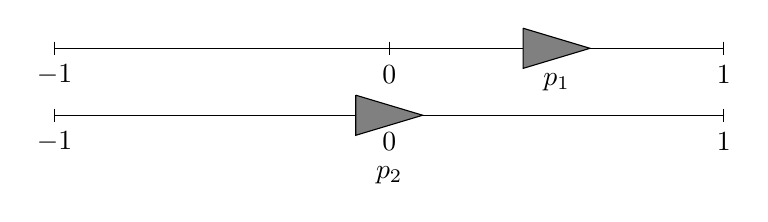
\begin{tikzpicture}[scale=0.85]
        % Dibujar el segmento de -1 a 1
        \draw[-] (-5,0) -- (5,0);
        
        % Poner las etiquetas en los extremos y en el centro
        \node at (-5, -0.4) {$-1$};
        \node at (0, -0.4) {$0$};
        \node at (5, -0.4) {$1$};
        
        % Poner las marcas en los puntos -1, 0 y 1
        \draw[-] (-5,0.1) -- (-5,-0.1);
        \draw[-] (0,0.1) -- (0,-0.1);
        \draw[-] (5,0.1) -- (5,-0.1);

        % Dron 1
        \draw[fill=gray,cm={cos(0),-sin(0),sin(0),cos(0),(0,0)}](2,0.3)--(2,-0.3)--(3,0)--(2,0.3);
        \node at (2.5, -0.5) {$p_1$};
        
        % Segundo Segmento
        % Dibujar el segmento de -1 a 1
        \draw[-] (-5,-1) -- (5,-1);
        
        % Poner las etiquetas en los extremos y en el centro
        \node at (-5, -1.4) {$-1$};
        \node at (0, -1.4) {$0$};
        \node at (5, -1.4) {$1$};
        
        % Poner las marcas en los puntos -1, 0 y 1
        \draw[-] (-5,-0.9) -- (-5,-1.1);
        \draw[-] (0,-0.9) -- (0,-1.1);
        \draw[-] (5,-0.9) -- (5,-1.1);

        % Dron 2
        \draw[fill=gray,cm={cos(0),-sin(0),sin(0),cos(0),(0,0)}](-0.5,-0.7)--(-0.5,-1.3)--(0.5,-1)--(-0.5,-0.7);
        \node at (0, -1.9) {$p_2$};
    \end{tikzpicture}
    \caption{Situación inicial para el ejemplo descrito de formación en segmentos}
    \label{fig:parallel-segments-formation-example}
\end{figure}

\subsubsection{Ajuste de la ganancia}

Al ser este algoritmo diseñado por el autor para este TFG, se propone la siguiente
forma de ajustar la ganancia:

\begin{itemize}
    \item Se supone $N = 2$ y $p^{*}_{ij} = 0$
    \item Se recomienda que la velocidad \textbf{mínima} de un dron sea 0 ($v_i = 0$). 
    En base a esto, el resultado de $K(p_j - p_i)$ deberá ser, 
    \textbf{como máximo} igual a $-v_n$
    \item Se sabe que, como máximo, $p_j - p_i = \pm 2$
\end{itemize}

En base a todo esto, podemos decir $0 = v_n - 2K$ que da 
como resultado $K = \frac{v_n}{2}$, por tanto, 
se recomienda usar una $K$ que sea la mitad de la velocidad nominal deseada.
La velocidad máxima será $v_i = v_n + Kmax(p_j - p_i) = v_n + 2 \frac{v_n}{2} = 2v_n$

Evidentemente, este método es un ejemplo para ajustar la ganancia. 
En función de los resultados deseados se preferirá un método u otro para ajustarla,
pero no se recomienda reducirla ni aumentarla mucho más, al poder haber problemas. 

%%%%%%%%%%%%%%%%%%%%%%%%%%%%%%%%%%%%%%%%%%%%%%%%%%%%%%%%%%%%%%%%%%%%%%%%%%%%%%%%%%%%%%%%%%%%%%%%%%%%%%%%%%%%%%%%%
%%%%%%%%%%%%%%%%%%%%%%%%%%%%%%%%%%%%%%%%%%%%%%%%%%%%%%%%%%%%%%%%%%%%%%%%%%%%%%%%%%%%%%%%%%%%%%%%%%%%%%%%%%%%%%%%%
%%%%%%%%%%%%%%%%%%%%%%%%%%%%%%%%%%%%%%%%%%%%%%%%%%%%%%%%%%%%%%%%%%%%%%%%%%%%%%%%%%%%%%%%%%%%%%%%%%%%%%%%%%%%%%%%%

\subsection{Comparativa entre formaciones}

Aprovechando que ya se han explicado y entendido ambos algoritmos, es interesante
comparar ambos algoritmos para ver sus similitudes. Recordemos ambas ecuaciones:

\begin{align*}
    r_i &= r_i + k_r B_i e \\
    v_i &= v_n + K \sum_{j=1}^{N} (p_j - p_i - p^{*}_{ij})
\end{align*}

Nótese que se ha expandido la \autoref{eq:applied-control-action-circular-formation} usando
la \autoref{eq:control-action-circular-formation}.

Es evidente, que hay grandes similitudes. A grandes rasgos, pueden compararse de la siguiente forma:

\begin{itemize}
    \item $r_i$ equivale a $v_i$
    \item $k_r$ equivale a $K$. 
    La principal diferencia es que en segmentos solo hay una constante para todos,
    pero se podría intercambiar por una matriz de ganancias $k_{ij}$
    \item $e$ es equivalente a $p_j - p_i - p^{*}_{ij}$. De hecho, si expandimos,
    $e = z_k - z_k^*$
    \item $B_i$ equivale indirectamente a los distintas expresiones resultantes del sumatorio 
    para todos $p^{*}_{ij}$ (esto último se puede expresar como la matriz de deajustes deseados $p^*$)
\end{itemize}
%%%%%%%%%%%%%%%%%%%%%%%%%%%%%%%%%%%%%%%%%%%%%%%%%%%%%%%%%%%%%%%%%%%%%%%%%%%%%%%%%%%%%%%%%%%%%%%%%%%%%%%%%%%%%%%%%
%%%%%%%%%%%%%%%%%%%%%%%%%%%%%%%%%%%%%%%%%%%%%%%%%%%%%%%%%%%%%%%%%%%%%%%%%%%%%%%%%%%%%%%%%%%%%%%%%%%%%%%%%%%%%%%%%
%%%%%%%%%%%%%%%%%%%%%%%%%%%%%%%%%%%%%%%%%%%%%%%%%%%%%%%%%%%%%%%%%%%%%%%%%%%%%%%%%%%%%%%%%%%%%%%%%%%%%%%%%%%%%%%%%

\section{Implementación de los algoritmos de coordinación}

Similarmente a GVF, Paparazzi ya incluye formación circular, 
pero no esta adaptada a rotorcrafts \cite{paparazzi-circular-formation}.
Adaptar esto implica diversos cambios referidos al ámbito de los rotorcrafts 
que se verán en la siguiente subsección.

%%%%%%%%%%%%%%%%%%%%%%%%%%%%%%%%%%%%%%%%%%%%%%%%%%%%%%%%%%%%%%%%%%%%%%%%%%%%%%%%%%%%%%%%%%%%%%%%%%%%%%%%%%%%%%%%%
%%%%%%%%%%%%%%%%%%%%%%%%%%%%%%%%%%%%%%%%%%%%%%%%%%%%%%%%%%%%%%%%%%%%%%%%%%%%%%%%%%%%%%%%%%%%%%%%%%%%%%%%%%%%%%%%%
%%%%%%%%%%%%%%%%%%%%%%%%%%%%%%%%%%%%%%%%%%%%%%%%%%%%%%%%%%%%%%%%%%%%%%%%%%%%%%%%%%%%%%%%%%%%%%%%%%%%%%%%%%%%%%%%%

\subsection{Adaptación de formaciones circulares}

Paparazzi ya incluye formaciones circulares utilizando un script de Python ubicado en
\texttt{sw/ground\_segment/python/gvf} llamado \texttt{circularFormation.py}.
Este script, similarmente a GVF, no tiene adaptación para rotorcrafts. 
En resumen, el script consiste en:

\begin{itemize}
    \item Ejecución del script con un párametro obligatorio que sera un archivo JSON con parámetros deseados
    \item Lectura del archivo JSON para recabar ajustes cómo los IDs internos de los vehículos en Paparazzi
    \item Sincronización del script con la instancia actual de Paparazzi. Hasta que no se encuentre todos los IDs de los UAVs funcionando bajo GVF tipo círculo el script no se comenzará a ejecutar
    \item Lectura de la telemetría recibida por los UAVs, para conseguir información como la posición actual
    \item Cálculo del algoritmo, es decir, cálculo de los ángulos entre vehículos, errores... para poder calcular el radio deseado para cada dron
    \item Se devuelve la telemetría a través de la libreria de Paparazzi para Python que permite comunicarse con los UAVs
\end{itemize}

La estructura de un archivo JSON suele ser como la siguiente:

% En realidad es JSON, pero no voy a hacer un perfil, con C vale
\begin{lstlisting}[style=CodigoC]
{
  "ids": [1,2],
  "topology": [
    [ 1],
    [-1]
  ],
  "desired_intervehicle_angles_degrees": [0],
  "gain": 10,
  "desired_stationary_radius_meters": 80
}
\end{lstlisting}

Donde podemos ver los IDs de los vehículos, la topología deseada (matriz $B$), 
ángulo deseado entre vehículos ($z^*$), ganancia ($k_r$) y el radio base deseado ($r_i$).

Para conseguir que esto también funcione para rotorcrafts y por tanto los Crazyflie, 
se han hecho los siguientes cambios:

\begin{itemize}
    \item Se añade un nuevo parámetro obligatorio al ejecutar el script.
    Este parámetro será el tipo de vehículo utilizado, en este caso, hay dos opciones:
    \begin{itemize}
        \item \textbf{Fixedwing:} la ya implementada para aviones de ala fija
        \item \textbf{Rotorcraft:} la nueva implementación para drones como el Crazyflie
    \end{itemize}
    \item Internamente en el script, se añade una condición que hará que se suscriba a los mensajes
    de \texttt{NAVIGATION} o \texttt{ROTORCRAFT\_FP} en función de el tipo de UAV deseado.
    Estos mensajes de telemetría son los encargados de mandar las posiciones relativas 
    (respecto al punto de inicio) de los fixedwing y rotorcraft, respectivamente. 
\end{itemize}

El resto del algoritmo no depende de ningún parámetro extra que pueda ser exclusivo a un tipo de UAV u otro.
Consecuentemente, no se necesitan más adaptaciones para las formaciones circulares en rotorcrafts.

%%%%%%%%%%%%%%%%%%%%%%%%%%%%%%%%%%%%%%%%%%%%%%%%%%%%%%%%%%%%%%%%%%%%%%%%%%%%%%%%%%%%%%%%%%%%%%%%%%%%%%%%%%%%%%%%%
%%%%%%%%%%%%%%%%%%%%%%%%%%%%%%%%%%%%%%%%%%%%%%%%%%%%%%%%%%%%%%%%%%%%%%%%%%%%%%%%%%%%%%%%%%%%%%%%%%%%%%%%%%%%%%%%%
%%%%%%%%%%%%%%%%%%%%%%%%%%%%%%%%%%%%%%%%%%%%%%%%%%%%%%%%%%%%%%%%%%%%%%%%%%%%%%%%%%%%%%%%%%%%%%%%%%%%%%%%%%%%%%%%%

\subsection{Implementación de formaciones en segmentos}

En base a la ya implementada formación en circulos, se ha hecho un nuevo
programa en Python que implementa la formacion en segmentos, ya que Paparazzi no incluye este programa. 
Los cambios son:

\begin{itemize}
    \item Ajustes generales al script del estilo nombres de variables, parámetros de entrada, comentarios...
    \item Cambio del algoritmo y de las clases para adaptarse a segmentos
    \item Cambios en la telemetría para sacar otros datos necesarios
    \item Solo funciona para rotorcrafts, al seguir estos un segmento de mejor forma que un fixedwing
\end{itemize}

Además, se ha cambiado la estructura del archivo JSON levemente para adaptarse al script. Por ejemplo:

\begin{lstlisting}[style=CodigoC]
{
  "ids": [8,9],
  "desired_normalized_offset": [0],
  "nominal_speed": 0.25,
  "gain": 0.15
}
\end{lstlisting}

Por último, al no ser explicado en la teoría de este algoritmo, 
se muestra aquí el trozo de código que hace la normalización del segmento:

\begin{lstlisting}[style=CodigoPython]
# Segment normalization
i = 0
for ac in self.aircraft:
    # Calculate x and y distances, from segment and current pos
    max_dist_x = ac.WP2[0] - ac.WP1[0]
    max_dist_y = ac.WP2[1] - ac.WP1[1]
    dist_x = ac.XY[0] - ac.WP1[0]
    dist_y = ac.XY[1] - ac.WP1[1]

    # Vector modulus (Pythagoras)
    max_dist = math.sqrt(max_dist_x**2 + max_dist_y**2)
    dist = math.sqrt(dist_x**2 + dist_y**2)

    # Having this, we can normalize the distance from 0 to 1
    norm_dist = dist / max_dist

    # Map segment values from range(0, 1) to range(-1, 1)
    def map_range(d, in_min, in_max, out_min, out_max):
        if (in_max == in_min):
            return 0
        else:
            return (d - in_min) * (out_max - out_min) / (in_max - in_min) + out_min
    
    self.mapped_pos[i] = map_range(norm_dist, 0, 1, -1, 1)
    i += 1
\end{lstlisting}

En resumen:

\begin{itemize}
    \item Se calculan las distancias en X y en Y
    \item Se calcula el módulo del vector de las distancias
    \item Se normaliza a 1
    \item Por último, se realiza un \textit{mapping} del vector normalizado (0 a 1) a la normalización propia (-1 a 1)
\end{itemize}

Evidentemente, existen más metodos para conseguir esta normalización (u otros tipos de normalización), 
pero se ha optado por este al ser simple de realizar, bajo coste computacional y fácil de entender. 
Funciona además, para un segmento en cualquier ángulo y dirección.

%%%%%%%%%%%%%%%%%%%%%%%%%%%%%%%%%%%%%%%%%%%%%%%%%%%%%%%%%%%%%%%%%%%%%%%%%%%%%%%%%%%%%%%%%%%%%%%%%%%%%%%%%%%%%%%%%
%%%%%%%%%%%%%%%%%%%%%%%%%%%%%%%%%%%%%%%%%%%%%%%%%%%%%%%%%%%%%%%%%%%%%%%%%%%%%%%%%%%%%%%%%%%%%%%%%%%%%%%%%%%%%%%%%
%%%%%%%%%%%%%%%%%%%%%%%%%%%%%%%%%%%%%%%%%%%%%%%%%%%%%%%%%%%%%%%%%%%%%%%%%%%%%%%%%%%%%%%%%%%%%%%%%%%%%%%%%%%%%%%%%

\section{Simulación de las formaciones}

Para acabar este capítulo, veremos los resultados en simulación de los algoritmos implementados.
Se verá tanto formaciones circulares como en segmentos. 
En el caso de las circulares, se obviará los casos reales ya que Paparazzi 
no permite realizar circulos de menos de 1 metro de diámetro. Esto último es difícil
de realizar en espacios interiores (los Crazyflies no funcionan correctamente en exteriores
debido a su bajo peso y, por tanto, el efecto del viento sobre estos)

%%%%%%%%%%%%%%%%%%%%%%%%%%%%%%%%%%%%%%%%%%%%%%%%%%%%%%%%%%%%%%%%%%%%%%%%%%%%%%%%%%%%%%%%%%%%%%%%%%%%%%%%%%%%%%%%%
%%%%%%%%%%%%%%%%%%%%%%%%%%%%%%%%%%%%%%%%%%%%%%%%%%%%%%%%%%%%%%%%%%%%%%%%%%%%%%%%%%%%%%%%%%%%%%%%%%%%%%%%%%%%%%%%%
%%%%%%%%%%%%%%%%%%%%%%%%%%%%%%%%%%%%%%%%%%%%%%%%%%%%%%%%%%%%%%%%%%%%%%%%%%%%%%%%%%%%%%%%%%%%%%%%%%%%%%%%%%%%%%%%%

\subsection{Simulación de formaciones circulares}

Se ha utilizado el siguiente archivo JSON:

\begin{lstlisting}[style=CodigoC]
{
  "ids": [8,9],
  "topology": [
    [ 1],
    [-1]
  ],
  "desired_intervehicle_angles_degrees": [0],
  "gain": 12,
  "desired_stationary_radius_meters": 75
}
\end{lstlisting}

Y se ha lanzado el script con los siguientes parámetros:

\begin{lstlisting}[style=CodigoBash]
python circularFormation.py formation/circular_two_bebops.json rotorcraft -v
\end{lstlisting}

Los resultados tras unos 500 segundos de simulación han sido los siguientes:

\begin{figure}[!h]
    \centering
    \includegraphics[width=0.99\textwidth]{img/fig/fig4.3-circular-formation-simulation-sample.png}
    \caption{Ejemplo de simulación de formaciones circulares con drones. 
    Se solapan ambos drones, al estar (como se desea) a 0 grados de error entre ambos}
    \label{fig:circular-formation-simulation}
\end{figure}

Además el error del ángulo a lo largo del tiempo ha sido el siguiente. 
Se parte de ambos haciendo GVF en un radio de unos 80 metros, con un error inicial entre ángulos de unos -6 grados sexagesimales:

\begin{figure}[h]
    \centering
    \includegraphics[width=0.99\textwidth]{img/fig/fig4.4-circular-formation-graph-error.png}
    \caption{Ángulo entre drones en simulación de formación circular. 
    En \textcolor{red}{rojo} el ángulo entre drones deseado}
    \label{fig:circular-formation-graph-error}
\end{figure}

Cómo podemos ver, converge lentamente a cerca de 0 grados de error.
No se termina de llegar a 0 ya que tomaría mucho tiempo, debido a que $k$ es aparentemente bajo para este escenario.

Tras esto, se mantiene estable en aproximadamente $\pm 1^o$ sexagesimales de error entre ambos drones.

%%%%%%%%%%%%%%%%%%%%%%%%%%%%%%%%%%%%%%%%%%%%%%%%%%%%%%%%%%%%%%%%%%%%%%%%%%%%%%%%%%%%%%%%%%%%%%%%%%%%%%%%%%%%%%%%%
%%%%%%%%%%%%%%%%%%%%%%%%%%%%%%%%%%%%%%%%%%%%%%%%%%%%%%%%%%%%%%%%%%%%%%%%%%%%%%%%%%%%%%%%%%%%%%%%%%%%%%%%%%%%%%%%%
%%%%%%%%%%%%%%%%%%%%%%%%%%%%%%%%%%%%%%%%%%%%%%%%%%%%%%%%%%%%%%%%%%%%%%%%%%%%%%%%%%%%%%%%%%%%%%%%%%%%%%%%%%%%%%%%%

\subsection{Simulación de formaciones en segmentos}

Se ha utilizado el siguiente archivo JSON:

\begin{lstlisting}[style=CodigoC]
{
  "ids": [8,9],
  "desired_normalized_offset": [0],
  "nominal_speed": 0.25,
  "gain": 0.18
}
\end{lstlisting}

Y se ha lanzado el script con los siguientes parámetros:

\begin{lstlisting}[style=CodigoBash]
python segmentFormation.py formation/segment/segment_two_bebops.json -v
\end{lstlisting}

En esta captura podemos ver dos drones en segmentos paralelos coordinados a la misma distancia en el segmento, es decir, sobre el mismo punto normalizado dentro del segmento (aproximadamente sobre 0.1):

\begin{figure}[!h]
    \centering
    \includegraphics[width=\textwidth]{img/fig/fig4.5-segment-formation-sim.png}
    \caption{Simulación de formación en segmentos en Paparazzi. 
    Podemos ver los drones que están al lado y en paralelo}
    \label{fig:segment-formation-simulation}
\end{figure}

Además el error en la posición del segmento normalizado a lo largo del tiempo ha sido la siguiente.
Se parte de ambos haciendo GVF para segmentos con un desajuste inicial aproximado de entre -0.5 y 0.5 (según instante de tiempo):

\begin{figure}[!h]
    \centering
    \includegraphics[width=\textwidth]{img/fig/fig4.6-segment-formation-graph-error.png}
    \caption{Desajuste de la posición sobre el segmento normalizado entre drones en simulación. En \textcolor{red}{rojo} el desajuste deseado}
    \label{fig:segment-formation-graph-error}
\end{figure}

Similarmente a formaciones circulares se converge lentamente a 0 de error, 
es decir, que uno este al lado del otro. Tras estabilizarse, el error no suele superar los $\pm 0.05$ sobre los segmentos normalizados, exceptuando en los extremos de los segmentos, que se suele ganar algo de error. 

%%%%%%%%%%%%%%%%%%%%%%%%%%%%%%%%%%%%%%%%%%%%%%%%%%%%%%%%%%%%%%%%%%%%%%%%%%%%%%%%%%%%%%%%%%%%%%%%%%%%%%%%%%%%%%%%%
%%%%%%%%%%%%%%%%%%%%%%%%%%%%%%%%%%%%%%%%%%%%%%%%%%%%%%%%%%%%%%%%%%%%%%%%%%%%%%%%%%%%%%%%%%%%%%%%%%%%%%%%%%%%%%%%%
%%%%%%%%%%%%%%%%%%%%%%%%%%%%%%%%%%%%%%%%%%%%%%%%%%%%%%%%%%%%%%%%%%%%%%%%%%%%%%%%%%%%%%%%%%%%%%%%%%%%%%%%%%%%%%%%%

\section{Coordinación y formación de Crazyflies}

Por último, se han de probar los experimentos de simulación en los Crazyflies reales.
Como se ha explicado previamente, se van a obviar los experimentos de formaciones circulares ya que no se dispone de un buen lugar para estos experimentos. 

%%%%%%%%%%%%%%%%%%%%%%%%%%%%%%%%%%%%%%%%%%%%%%%%%%%%%%%%%%%%%%%%%%%%%%%%%%%%%%%%%%%%%%%%%%%%%%%%%%%%%%%%%%%%%%%%%
%%%%%%%%%%%%%%%%%%%%%%%%%%%%%%%%%%%%%%%%%%%%%%%%%%%%%%%%%%%%%%%%%%%%%%%%%%%%%%%%%%%%%%%%%%%%%%%%%%%%%%%%%%%%%%%%%
%%%%%%%%%%%%%%%%%%%%%%%%%%%%%%%%%%%%%%%%%%%%%%%%%%%%%%%%%%%%%%%%%%%%%%%%%%%%%%%%%%%%%%%%%%%%%%%%%%%%%%%%%%%%%%%%%

\subsection{Comparación entre firmware oficial y de Paparazzi}

Las primeras pruebas resultaron ser prometedoras, pero no suficiente, ya que el Flow Deck, aunque mejor que la IMU sola, 
acumula suficiente error como para que antes de que se coordinen ambos drones se choquen o desvíen demasiado del objetivo, sin llegar a coordinarse. 
En otras palabras, se puede realizar GVF y/o coordinación bajo un tiempo límite si se utiliza posición relativa, 
pero la coordinación necesita más de ese tiempo límite. 
Aquí es un buen ejemplo donde el Loco Positioning System explicado en el capítulo 1 hubiese ayudado, 
pero se descartó finalmente por falta de un lugar apropiado donde instalarlo.

Consecuentemente, se probó con el firmware de Bitcraze (que se utilizó en el capítulo 2) la estabilidad a lo largo del tiempo y resultó ser considerablemente mayor. 
En otras palabras, el ajuste de estabilización del PID y lectura de los sensores es \textbf{claramente superior en el firmware oficial a en Paparazzi}. En resumen:

\begin{itemize}
    \item El firmware de Paparazzi es superior en versatilidad, opciones de módulos, telemetría... y es capaz de hacer simulaciones.
    \item Por contraparte, el firmware de Bitcraze es superior en control del Crazyflie, facilidad de uso (tanto programación como uso general) y documentación.
\end{itemize}

Por ello, tras demostrar la viabilidad del algoritmo en simulación, se va a realizar la demostración de la coordinación \textbf{bajo el firmware oficial de Bitcraze}.

%%%%%%%%%%%%%%%%%%%%%%%%%%%%%%%%%%%%%%%%%%%%%%%%%%%%%%%%%%%%%%%%%%%%%%%%%%%%%%%%%%%%%%%%%%%%%%%%%%%%%%%%%%%%%%%%%
%%%%%%%%%%%%%%%%%%%%%%%%%%%%%%%%%%%%%%%%%%%%%%%%%%%%%%%%%%%%%%%%%%%%%%%%%%%%%%%%%%%%%%%%%%%%%%%%%%%%%%%%%%%%%%%%%
%%%%%%%%%%%%%%%%%%%%%%%%%%%%%%%%%%%%%%%%%%%%%%%%%%%%%%%%%%%%%%%%%%%%%%%%%%%%%%%%%%%%%%%%%%%%%%%%%%%%%%%%%%%%%%%%%

\subsection{Control en el firmware de Bitcraze}

Para entender mejor esta subsección y las siguientes,
se recomienda leer paralelamente el \autoref{appendix:user_manual},
concretamente la sección para Bitcraze. Veamos un script de ejemplo:

\begin{lstlisting}[style=CodigoPython]
# crazyflie_demo.py
# ...

import cflib.crtp
from cflib.crazyflie import Crazyflie
from cflib.crazyflie.syncCrazyflie import SyncCrazyflie
from cflib.positioning.motion_commander import MotionCommander
from cflib.utils import uri_helper

URI = uri_helper.uri_from_env(default='radio://0/80/2M/E7E7E7E701')
DEFAULT_HEIGHT = 0.5

# ...

def move_linear_simple(scf):
    with MotionCommander(scf, default_height=DEFAULT_HEIGHT) as mc:
        time.sleep(1)
        mc.forward(0.5)
        time.sleep(1)
        mc.turn_left(180)
        time.sleep(1)
        mc.forward(0.5)
        time.sleep(1)

# ...

if __name__ == '__main__':
    cflib.crtp.init_drivers()

    with SyncCrazyflie(URI, cf=Crazyflie(rw_cache='./cache')) as scf:
        # ...
        move_linear_simple(scf)
\end{lstlisting}

\textbf{\texttt{\# ...} representa fragmentos de código que no se han escrito} 
porque no son necesarios para entender la totalidad del código.

Cómo podemos ver en el fragmento de código anterior, 
el control de un Crazyflie es trivial en comparación con Paparazzi.
El ajuste de PID, los diversos módulos, la necesidad de recompilar el firmware...
todo esta abstraído de forma que pueda ser más simple el control básico.

A grandes rasgos, tan sólo hay que inicializar los drivers, 
crear el objeto \texttt{scf} para control del Crazyflie y llamar a una función que indica que se va a comandar.
En la función tan sólo hay que indicar si se quiere ir hacia delante, atrás, rotar...
Por supuesto existen otros métodos de control, por ejemplo, dirigirse hacia cierta posición, o comandar
directamente el roll, pitch, yaw y throttle.

%%%%%%%%%%%%%%%%%%%%%%%%%%%%%%%%%%%%%%%%%%%%%%%%%%%%%%%%%%%%%%%%%%%%%%%%%%%%%%%%%%%%%%%%%%%%%%%%%%%%%%%%%%%%%%%%%
%%%%%%%%%%%%%%%%%%%%%%%%%%%%%%%%%%%%%%%%%%%%%%%%%%%%%%%%%%%%%%%%%%%%%%%%%%%%%%%%%%%%%%%%%%%%%%%%%%%%%%%%%%%%%%%%%
%%%%%%%%%%%%%%%%%%%%%%%%%%%%%%%%%%%%%%%%%%%%%%%%%%%%%%%%%%%%%%%%%%%%%%%%%%%%%%%%%%%%%%%%%%%%%%%%%%%%%%%%%%%%%%%%%

\subsection{Formación en segmentos en el firmware de Bitcraze}

Para implementar el algoritmo de coordinación sobre el firmware oficial, 
se ha decidio obviar GVF ya que, aunque es preferible debido al buen control que ofrece,
no es necesario para hacer una demostración del algoritmo de coordinación.
Por ello la implementación de la coordinación en segmentos se ha realizado de la siguiente forma \cite{crazyradio-swarm-interface}:

\begin{lstlisting}[style=CodigoPython]
# crazyflie_segment_formation.py
# ...

uris = {
    'radio://0/80/2M/E7E7E7E701',
    'radio://0/80/2M/E7E7E7E702',
}

waiting_uri = 'radio://0/80/2M/E7E7E7E702' # Crazyflie that waits
all_positions = {}

NOMINAL_SPEED = [0.2, 0] # x, y respectively
DEFAULT_HEIGHT = 0.5 # In meters
SEGMENT_LIMIT = 1 # Meters
FREQ = 0.2 # How many seconds until we update the speed

# ...

def kuramoto(my_position, other_positions):
    k = 0.12
    desired_offset = 0

    delta = 0
    for position in other_positions:
        delta += position[0] - my_position[0] - desired_offset
    
    return k * delta

def get_xy_from(radio, positions):
    return (positions[radio].x, positions[radio].y)
    
def coordinated_segment(scf):
    with MotionCommander(scf, default_height=DEFAULT_HEIGHT) as mc:
        my_nominal_speed = {}
        my_nominal_speed[scf._link_uri] = NOMINAL_SPEED
        
        # ...

        while True:
            # First we calculate positions
            my_position = get_xy_from(scf._link_uri, all_positions)

            # Calculate every other drone position
            other_positions = []
            for uri in uris:
                if uri != scf._link_uri:
                    other_positions.append(get_xy_from(uri, all_positions))

            # Change direction if passed the limit
            if my_position[0] > SEGMENT_LIMIT:
                my_nominal_speed[scf._link_uri][0] = -NOMINAL_SPEED[0]
            elif my_position[0] < -SEGMENT_LIMIT:
                my_nominal_speed[scf._link_uri][0] = NOMINAL_SPEED[0]

            speed_x = my_nominal_speed[scf._link_uri][0]
            
            # Add Kuramoto speed
            speed_x += kuramoto(my_position, other_positions)

            mc.start_linear_motion(speed_x, speed_y, 0)
            time.sleep(FREQ)

def recover_positions():
    global all_positions
    while True:
        all_positions = swarm.get_estimated_positions()
        time.sleep(FREQ / 2)

if __name__ == '__main__':
    # ...
    with Swarm(uris, factory=factory) as swarm:        
        # ...
        recover_positions_thread.start()
        swarm.parallel(coordinated_segment)
        # ...
\end{lstlisting}

Similarmente al ejemplo anterior, \textbf{\texttt{\# ...} representa trozos de código que se han obviado} al no ser
relevantes para entender la funcionalidad principal.

Podemos dividir el código en las siguientes secciones:

\begin{itemize}
    \item \texttt{recover\_positions()}: función que se ocupa de recuperar las posiciones de los drones 
    cada \texttt{FREQ / 2} segundos. Se ejecuta en un thread aparte.
    \item \texttt{kuramoto()}: recibe las posiciones de todos los drones y calcula para cada dron cuanto debe
    aumentar o reducir su velocidad con el algoritmo para segmentos paralelos.
    \item \texttt{coordinated\_segment():} función principal para coordinar los drones.
    Calcula posiciones, invierte la velocidad lineal de un dron si ha pasado del segmento y 
    comanda la velocidad calculada por el algoritmo cada \texttt{FREQ} segundos.
\end{itemize}

En general, esta implementación simplificada sigue un segmento en X sin importar su posición en Y.
Su dirección cambiará cuando llegue a 1 metro y cuando llegue a -1 metro, permitiendo obviar la normalización.
Si bien puede ser simple, el objetivo final que es aplicar el algoritmo, se puede conseguir igualmente.

%%%%%%%%%%%%%%%%%%%%%%%%%%%%%%%%%%%%%%%%%%%%%%%%%%%%%%%%%%%%%%%%%%%%%%%%%%%%%%%%%%%%%%%%%%%%%%%%%%%%%%%%%%%%%%%%%
%%%%%%%%%%%%%%%%%%%%%%%%%%%%%%%%%%%%%%%%%%%%%%%%%%%%%%%%%%%%%%%%%%%%%%%%%%%%%%%%%%%%%%%%%%%%%%%%%%%%%%%%%%%%%%%%%
%%%%%%%%%%%%%%%%%%%%%%%%%%%%%%%%%%%%%%%%%%%%%%%%%%%%%%%%%%%%%%%%%%%%%%%%%%%%%%%%%%%%%%%%%%%%%%%%%%%%%%%%%%%%%%%%%

\subsection{Resultados de la coordinación}

Ejecutando el programa mostrado en la subsección anterior, los resultados fueron prometedores: 
el algoritmo funciona correctamente, pero actualmente hay un error en el código de Bitcraze que impiden que se den la vuelta correctamente en el segmento.

\begin{figure}[h]
    \centering
    \includegraphics[width=\textwidth]{img/fig/fig4.7-coordinated-crazyflies.jpg}
    \caption{Dos drones manteniéndose paralelos. 
    En este caso $p^* = 0, \ v_n = 0.2 \ m/s, \ K = 0.12$}
    \label{fig:coordinated-crazyflies}
\end{figure}

Para verificar que esto no es culpa de un error en la programación o algoritmo,
se ha decidido añadir un último experimento que utiliza un log real de un sólo dron siguiendo un segmento y 
un dron simulado aplicando el algoritmo en base a las posiciones reales del log, 
es decir, tratando de mantenerse coordinado con las posiciones del dron real guardadas en el log.
Mas información de este experimento en el \autoref{appendix:user_manual}.

Para este experimento:

\begin{itemize}
    \item $p^* = 0, \ v_n = 0.1 \ m/s$. 
    Para el caso del log sacado del dron real, se mantuvo una velocidad fija de $0.1 \ m/s$.
    \item Se fijo un segmento con posiciones $(-0.5, 0)$ y $(0.5, 0)$, es decir,
    para este caso no se normalizó el segmento. 
    Consecuentemente,  se ha decidido que $K = 0.3$ (3 veces más alto que la velocidad nominal), 
    para compensar por el hecho de que el segmento es más corto. 
    \item También, se ha elegido un valor de $K$ más alto para que se pueda mantener más cerca el dron simulado del real, ya que al ser una simulación controlado se pueden evitar los posibles errores de elegir un $K$ alto.
    \item Por último, se ha decidido fijar las posiciones en el eje Y. 
    En el caso del dron real hubo una ligera variación, pero por simplificar, se ha asumido que los valores de $p_y$ fueron constantes.
\end{itemize}

\begin{figure}[h]
    \centering
    \includegraphics[width=\textwidth]{img/fig/fig4.8-coordinated-experiment.png}
    \caption{Animación del experimento que verifica que el algoritmo funciona}
    \label{fig:coordination-experiment}
\end{figure}

En la siguiente figura podemos ver el error de la posición entre los drones. 
Se obvian los dos primeros segundos que el dron simulado esta quieto:

\begin{figure}[h]
    \centering
    \includegraphics[width=\textwidth]{img/fig/fig4.9-experiment-pos-error.png}
    \caption{Diferencia de la posición entre los drones. 
    En \textcolor{Green3}{verde} la diferencia deseado}
    \label{fig:pos-error-experiment}
\end{figure}

Podemos ver que el error no sube de 0.1 m tras estabilizarse.
Si obviamos los máximos locales (se producen al dar la vuelta en el segmento), el error esta típicamente por debajo de 0.05 m, es decir por debajo del $10\%$ de error.

Por último, la velocidad del dron simulado fue la siguiente (para los mismos instantes de tiempo):

\begin{figure}[h]
    \centering
    \includegraphics[width=\textwidth]{img/fig/fig4.10-experiment-speed.png}
    \caption{Velocidad del dron rojo (simulado). 
    En \textcolor{Green3}{verde} la velocidad nominal objetivo en ese instante}
    \label{fig:speed-experiment}
\end{figure}

Es interesante ver los bruscos cambios, al ser un dron simulado sin GVF.

Este experimento también sirve para entender las impresionantes capacidades de Paparazzi para simulación.
Es evidente que para ello, Paparazzi es superior a otras alternativas software,
en especial para los Crazyflies, que no dispone de una extensa variedad.

Finalmente, se recomienda para ambos experimentos ver las animaciones y vídeos correspondientes en la presentación por diapositivas de este TFG para entender mejor los resultados que en las figuras \cite{final-results}. 